\documentclass{book}
\usepackage[a4paper,top=2.5cm,bottom=2.5cm,left=2.5cm,right=2.5cm]{geometry}
\usepackage{makeidx}
\usepackage{natbib}
\usepackage{graphicx}
\usepackage{multicol}
\usepackage{float}
\usepackage{listings}
\usepackage{color}
\usepackage{ifthen}
\usepackage[table]{xcolor}
\usepackage{textcomp}
\usepackage{alltt}
\usepackage{ifpdf}
\ifpdf
\usepackage[pdftex,
            pagebackref=true,
            colorlinks=true,
            linkcolor=blue,
            unicode
           ]{hyperref}
\else
\usepackage[ps2pdf,
            pagebackref=true,
            colorlinks=true,
            linkcolor=blue,
            unicode
           ]{hyperref}
\usepackage{pspicture}
\fi
\usepackage[utf8]{inputenc}
\usepackage[french]{babel}

\usepackage{mathptmx}
\usepackage[scaled=.90]{helvet}
\usepackage{courier}
\usepackage{sectsty}
\usepackage{amssymb}
\usepackage[titles]{tocloft}
\usepackage{doxygen}
\lstset{language=C++,inputencoding=utf8,basicstyle=\footnotesize,breaklines=true,breakatwhitespace=true,tabsize=4,numbers=left }
\makeindex
\setcounter{tocdepth}{3}
\renewcommand{\footrulewidth}{0.4pt}
\renewcommand{\familydefault}{\sfdefault}
\hfuzz=15pt
\setlength{\emergencystretch}{15pt}
\hbadness=750
\tolerance=750
\begin{document}
\hypersetup{pageanchor=false,citecolor=blue}
\begin{titlepage}
\vspace*{7cm}
\begin{center}
{\Large Creuvux }\\
\vspace*{1cm}
{\large Généré par Doxygen 1.8.3.1}\\
\vspace*{0.5cm}
{\small Mercredi Février 27 2013 20:48:19}\\
\end{center}
\end{titlepage}
\clearemptydoublepage
\pagenumbering{roman}
\tableofcontents
\clearemptydoublepage
\pagenumbering{arabic}
\hypersetup{pageanchor=true,citecolor=blue}
\chapter{Index des structures de données}
\section{Structures de données}
Liste des structures de données avec une brève description \-:\begin{DoxyCompactList}
\item\contentsline{section}{\hyperlink{struct_command__options}{Command\-\_\-options} }{\pageref{struct_command__options}}{}
\item\contentsline{section}{\hyperlink{struct_gstat}{Gstat} }{\pageref{struct_gstat}}{}
\item\contentsline{section}{\hyperlink{struct_server_options}{Server\-Options} }{\pageref{struct_server_options}}{}
\item\contentsline{section}{\hyperlink{structslist__t}{slist\-\_\-t} }{\pageref{structslist__t}}{}
\item\contentsline{section}{\hyperlink{structstring__t}{string\-\_\-t} }{\pageref{structstring__t}}{}
\item\contentsline{section}{\hyperlink{struct_ustat}{Ustat} }{\pageref{struct_ustat}}{}
\end{DoxyCompactList}

\chapter{Index des fichiers}
\section{Liste des fichiers}
Liste de tous les fichiers documentés avec une brève description \-:\begin{DoxyCompactList}
\item\contentsline{section}{{\bfseries create\-\_\-database.\-h} }{\pageref{create__database_8h}}{}
\item\contentsline{section}{\hyperlink{creuvard_8c}{creuvard.\-c} \\*Fonction interne }{\pageref{creuvard_8c}}{}
\item\contentsline{section}{{\bfseries creuvard.\-h} }{\pageref{creuvard_8h}}{}
\item\contentsline{section}{{\bfseries creuvux\-\_\-stat.\-h} }{\pageref{creuvux__stat_8h}}{}
\item\contentsline{section}{\hyperlink{creuvuxd_8c}{creuvuxd.\-c} \\*Fichier principale }{\pageref{creuvuxd_8c}}{}
\item\contentsline{section}{{\bfseries crv\-\_\-mysql.\-h} }{\pageref{crv__mysql_8h}}{}
\item\contentsline{section}{{\bfseries crv\-\_\-string.\-h} }{\pageref{crv__string_8h}}{}
\item\contentsline{section}{{\bfseries get.\-h} }{\pageref{get_8h}}{}
\item\contentsline{section}{{\bfseries help.\-h} }{\pageref{help_8h}}{}
\item\contentsline{section}{{\bfseries log.\-h} }{\pageref{log_8h}}{}
\item\contentsline{section}{{\bfseries network.\-h} }{\pageref{network_8h}}{}
\item\contentsline{section}{{\bfseries put.\-h} }{\pageref{put_8h}}{}
\item\contentsline{section}{\hyperlink{server__conf_8c}{server\-\_\-conf.\-c} \\*Fichier contenant 2 fonctions de configurations du serveur }{\pageref{server__conf_8c}}{}
\item\contentsline{section}{{\bfseries server\-\_\-conf.\-h} }{\pageref{server__conf_8h}}{}
\item\contentsline{section}{{\bfseries S\-S\-L\-\_\-loadfile.\-h} }{\pageref{_s_s_l__loadfile_8h}}{}
\item\contentsline{section}{{\bfseries S\-S\-L\-\_\-sendfile.\-h} }{\pageref{_s_s_l__sendfile_8h}}{}
\item\contentsline{section}{{\bfseries sync.\-h} }{\pageref{sync_8h}}{}
\item\contentsline{section}{{\bfseries update\-\_\-database.\-h} }{\pageref{update__database_8h}}{}
\end{DoxyCompactList}

\chapter{Documentation des structures de données}
\hypertarget{struct_command__options}{\section{Référence de la structure Command\-\_\-options}
\label{struct_command__options}\index{Command\-\_\-options@{Command\-\_\-options}}
}
\subsection*{Champs de données}
\begin{DoxyCompactItemize}
\item 
\hypertarget{struct_command__options_a5ac083a645d964373f022d03df4849c8}{char $\ast$ {\bfseries name}}\label{struct_command__options_a5ac083a645d964373f022d03df4849c8}

\item 
\hypertarget{struct_command__options_a56abfaab87c46691c1ef3ad0df23e864}{char $\ast$ {\bfseries version}}\label{struct_command__options_a56abfaab87c46691c1ef3ad0df23e864}

\item 
\hypertarget{struct_command__options_a6890c4a9b97760f22db3acd8c7c6c81e}{off\-\_\-t {\bfseries begin}}\label{struct_command__options_a6890c4a9b97760f22db3acd8c7c6c81e}

\item 
\hypertarget{struct_command__options_a6b744082ecd6f39e8b56e8d7d6413499}{off\-\_\-t {\bfseries end}}\label{struct_command__options_a6b744082ecd6f39e8b56e8d7d6413499}

\item 
\hypertarget{struct_command__options_a469f221a5d0a0abb4ce4526d185b9740}{char $\ast$ {\bfseries grp}}\label{struct_command__options_a469f221a5d0a0abb4ce4526d185b9740}

\item 
\hypertarget{struct_command__options_adf916204820072417ed73a32de1cefcf}{int {\bfseries flag}}\label{struct_command__options_adf916204820072417ed73a32de1cefcf}

\item 
\hypertarget{struct_command__options_aa0e04e47800a4ae6a856f0fdb5426215}{char $\ast$ {\bfseries addr}}\label{struct_command__options_aa0e04e47800a4ae6a856f0fdb5426215}

\item 
\hypertarget{struct_command__options_a14871705f45ccdc5bb9f4549efd8e119}{char $\ast$ {\bfseries user}}\label{struct_command__options_a14871705f45ccdc5bb9f4549efd8e119}

\item 
\hypertarget{struct_command__options_af236e8ba7815eda2ff7daf67c80043bb}{char $\ast$ {\bfseries mail}}\label{struct_command__options_af236e8ba7815eda2ff7daf67c80043bb}

\item 
\hypertarget{struct_command__options_ae08c24c84452c09a4d50e1a8ae5d963f}{char $\ast$ {\bfseries sha1}}\label{struct_command__options_ae08c24c84452c09a4d50e1a8ae5d963f}

\item 
\hypertarget{struct_command__options_a44196e6a5696d10442c29e639437196e}{char $\ast$ {\bfseries path}}\label{struct_command__options_a44196e6a5696d10442c29e639437196e}

\item 
\hypertarget{struct_command__options_a73d8ede97b4a863bb11c8225a5c8b70d}{char $\ast$ {\bfseries lst\-\_\-file}}\label{struct_command__options_a73d8ede97b4a863bb11c8225a5c8b70d}

\item 
\hypertarget{struct_command__options_aeac90097f29f7529968697163cea5c18}{char $\ast$ {\bfseries filename}}\label{struct_command__options_aeac90097f29f7529968697163cea5c18}

\item 
\hypertarget{struct_command__options_a43fdab0b6bb94ab25f7a2d2ee003146b}{char $\ast$ {\bfseries old\-\_\-sha1}}\label{struct_command__options_a43fdab0b6bb94ab25f7a2d2ee003146b}

\item 
\hypertarget{struct_command__options_afd39d2a5f0192a3836ea8e6a272430a3}{char $\ast$ {\bfseries genre}}\label{struct_command__options_afd39d2a5f0192a3836ea8e6a272430a3}

\item 
\hypertarget{struct_command__options_a25dae25c3bf9b28d54eb4df7afb2a491}{char $\ast$ {\bfseries comment}}\label{struct_command__options_a25dae25c3bf9b28d54eb4df7afb2a491}

\end{DoxyCompactItemize}


La documentation de cette structure a été générée à partir du fichier suivant \-:\begin{DoxyCompactItemize}
\item 
network.\-h\end{DoxyCompactItemize}

\hypertarget{struct_gstat}{\section{Référence de la structure Gstat}
\label{struct_gstat}\index{Gstat@{Gstat}}
}
\subsection*{Champs de données}
\begin{DoxyCompactItemize}
\item 
\hypertarget{struct_gstat_a1b3d4d20a7d1b8d3232a35dd689ecfc9}{int {\bfseries nb\-\_\-sync}}\label{struct_gstat_a1b3d4d20a7d1b8d3232a35dd689ecfc9}

\item 
\hypertarget{struct_gstat_a6c53f9a18d82d8b3eb69db87bebb5278}{int {\bfseries nb\-\_\-put}}\label{struct_gstat_a6c53f9a18d82d8b3eb69db87bebb5278}

\item 
\hypertarget{struct_gstat_a9c5fc500b4e111d67e3116a98fc0079a}{int {\bfseries nb\-\_\-get}}\label{struct_gstat_a9c5fc500b4e111d67e3116a98fc0079a}

\item 
\hypertarget{struct_gstat_a3b935650d378d427a56b873a84a80106}{int {\bfseries nb\-\_\-comment}}\label{struct_gstat_a3b935650d378d427a56b873a84a80106}

\item 
\hypertarget{struct_gstat_ab546ca1885cfe0cb636237597b6c03ea}{int {\bfseries nb\-\_\-tot}}\label{struct_gstat_ab546ca1885cfe0cb636237597b6c03ea}

\item 
\hypertarget{struct_gstat_ae2c60a5b9873f763ab7636ef25953c00}{off\-\_\-t {\bfseries size\-\_\-get}}\label{struct_gstat_ae2c60a5b9873f763ab7636ef25953c00}

\item 
\hypertarget{struct_gstat_a750fc6b8808d30cb4c5c262e2ae81e80}{off\-\_\-t {\bfseries size\-\_\-put}}\label{struct_gstat_a750fc6b8808d30cb4c5c262e2ae81e80}

\item 
\hypertarget{struct_gstat_a98544d36afdaaa3f139da8f248c2bb99}{off\-\_\-t {\bfseries size\-\_\-tot}}\label{struct_gstat_a98544d36afdaaa3f139da8f248c2bb99}

\item 
\hypertarget{struct_gstat_a33a60d65e3b7ae90db3421d39935178a}{off\-\_\-t {\bfseries size\-\_\-comment}}\label{struct_gstat_a33a60d65e3b7ae90db3421d39935178a}

\item 
\hypertarget{struct_gstat_a600b792d6d2ff2e71096dfa60d97a3b0}{F\-I\-L\-E $\ast$ {\bfseries fd}}\label{struct_gstat_a600b792d6d2ff2e71096dfa60d97a3b0}

\end{DoxyCompactItemize}


La documentation de cette structure a été générée à partir du fichier suivant \-:\begin{DoxyCompactItemize}
\item 
creuvux\-\_\-stat.\-c\end{DoxyCompactItemize}

\hypertarget{struct_server_options}{\section{Référence de la structure Server\-Options}
\label{struct_server_options}\index{Server\-Options@{Server\-Options}}
}
\subsection*{Champs de données}
\begin{DoxyCompactItemize}
\item 
\hypertarget{struct_server_options_af4b8906f613beba3ee0d5d835b157b9e}{int {\bfseries num\-\_\-ports}}\label{struct_server_options_af4b8906f613beba3ee0d5d835b157b9e}

\item 
\hypertarget{struct_server_options_a14871705f45ccdc5bb9f4549efd8e119}{char $\ast$ {\bfseries user}}\label{struct_server_options_a14871705f45ccdc5bb9f4549efd8e119}

\item 
\hypertarget{struct_server_options_a44196e6a5696d10442c29e639437196e}{char $\ast$ {\bfseries path}}\label{struct_server_options_a44196e6a5696d10442c29e639437196e}

\item 
\hypertarget{struct_server_options_a71b420b9a271ff67fe17d3f93d6a81b1}{int {\bfseries bandwidth}}\label{struct_server_options_a71b420b9a271ff67fe17d3f93d6a81b1}

\item 
\hypertarget{struct_server_options_a61814971ee95918cbf298473b56cfae4}{char $\ast$ {\bfseries chroot\-\_\-directory}}\label{struct_server_options_a61814971ee95918cbf298473b56cfae4}

\item 
\hypertarget{struct_server_options_a74bb62276efdf39dd94048e007fca05b}{char $\ast$ {\bfseries config}}\label{struct_server_options_a74bb62276efdf39dd94048e007fca05b}

\item 
\hypertarget{struct_server_options_ab4980c4af3d9844ee84d01622ac53e11}{char $\ast$ {\bfseries listen\-\_\-addrs}}\label{struct_server_options_ab4980c4af3d9844ee84d01622ac53e11}

\item 
\hypertarget{struct_server_options_a42ff4f2fd3b82ceab5c6785e7d66a6cb}{int {\bfseries address\-\_\-family}}\label{struct_server_options_a42ff4f2fd3b82ceab5c6785e7d66a6cb}

\item 
\hypertarget{struct_server_options_a1c2046dcb30a629d6d9f45ff8f403f12}{char $\ast$ {\bfseries host}}\label{struct_server_options_a1c2046dcb30a629d6d9f45ff8f403f12}

\item 
\hypertarget{struct_server_options_ac3e1795766a80ec63b157951b4b9a7d4}{int {\bfseries debug}}\label{struct_server_options_ac3e1795766a80ec63b157951b4b9a7d4}

\item 
\hypertarget{struct_server_options_aca2dbe38e002239b106d230253c0a1de}{char $\ast$ {\bfseries pid}}\label{struct_server_options_aca2dbe38e002239b106d230253c0a1de}

\item 
\hypertarget{struct_server_options_a90c2ace84e5523d06b7162ea5928acc1}{int {\bfseries sec}}\label{struct_server_options_a90c2ace84e5523d06b7162ea5928acc1}

\item 
\hypertarget{struct_server_options_a4abd489e86cf2b92d3a0e1fe86eaa28d}{char $\ast$ {\bfseries passphrase}}\label{struct_server_options_a4abd489e86cf2b92d3a0e1fe86eaa28d}

\item 
\hypertarget{struct_server_options_a40c6706b1ee653a8eabbf48d9503c633}{char $\ast$ {\bfseries upload\-\_\-directory}}\label{struct_server_options_a40c6706b1ee653a8eabbf48d9503c633}

\item 
\hypertarget{struct_server_options_abb449da8a584bb7fd1ebd6a04639603a}{char $\ast$ {\bfseries public\-\_\-directory}}\label{struct_server_options_abb449da8a584bb7fd1ebd6a04639603a}

\item 
\hypertarget{struct_server_options_a985249afc14c20d33d4ffbc32477a567}{char $\ast$ {\bfseries stat\-\_\-repport}}\label{struct_server_options_a985249afc14c20d33d4ffbc32477a567}

\item 
\hypertarget{struct_server_options_a7cc99031f6dcba96698be1186156776c}{off\-\_\-t {\bfseries db\-\_\-max}}\label{struct_server_options_a7cc99031f6dcba96698be1186156776c}

\item 
\hypertarget{struct_server_options_a6a03ec4a9049c9b45e35cf24922b229e}{off\-\_\-t {\bfseries db\-\_\-min}}\label{struct_server_options_a6a03ec4a9049c9b45e35cf24922b229e}

\item 
\hypertarget{struct_server_options_a40480c53ffec653b77bdc329c28b00b8}{char $\ast$ {\bfseries ipdb}}\label{struct_server_options_a40480c53ffec653b77bdc329c28b00b8}

\item 
\hypertarget{struct_server_options_a2d0838d497adbb90268461e9fb7011b5}{int $\ast$ {\bfseries portdb}}\label{struct_server_options_a2d0838d497adbb90268461e9fb7011b5}

\item 
\hypertarget{struct_server_options_aeb5780a92251203a659de23ac01f43f4}{char $\ast$ {\bfseries dbname}}\label{struct_server_options_aeb5780a92251203a659de23ac01f43f4}

\item 
\hypertarget{struct_server_options_afb39a000085218867ad6b0e6a027b374}{char $\ast$ {\bfseries dbuser}}\label{struct_server_options_afb39a000085218867ad6b0e6a027b374}

\item 
\hypertarget{struct_server_options_af9ffd0586c205c74ed2bd131e03e8b1c}{char $\ast$ {\bfseries dbpassw}}\label{struct_server_options_af9ffd0586c205c74ed2bd131e03e8b1c}

\end{DoxyCompactItemize}


La documentation de cette structure a été générée à partir du fichier suivant \-:\begin{DoxyCompactItemize}
\item 
server\-\_\-conf.\-h\end{DoxyCompactItemize}

\hypertarget{structslist__t}{\section{Référence de la structure slist\-\_\-t}
\label{structslist__t}\index{slist\-\_\-t@{slist\-\_\-t}}
}
\subsection*{Champs de données}
\begin{DoxyCompactItemize}
\item 
\hypertarget{structslist__t_a5ac083a645d964373f022d03df4849c8}{char $\ast$ {\bfseries name}}\label{structslist__t_a5ac083a645d964373f022d03df4849c8}

\item 
\hypertarget{structslist__t_ad39f70e6e4e7d93801b4810fb5138060}{int {\bfseries is\-\_\-dir}}\label{structslist__t_ad39f70e6e4e7d93801b4810fb5138060}

\item 
\hypertarget{structslist__t_a7c8ee186f75ca8d5f092b8e9f961dca3}{struct slist $\ast$ {\bfseries next}}\label{structslist__t_a7c8ee186f75ca8d5f092b8e9f961dca3}

\end{DoxyCompactItemize}


La documentation de cette structure a été générée à partir du fichier suivant \-:\begin{DoxyCompactItemize}
\item 
create\-\_\-database.\-c\end{DoxyCompactItemize}

\hypertarget{structstring__t}{\section{Référence de la structure string\-\_\-t}
\label{structstring__t}\index{string\-\_\-t@{string\-\_\-t}}
}
\subsection*{Champs de données}
\begin{DoxyCompactItemize}
\item 
\hypertarget{structstring__t_a3e6c64a4b8fd9c31b174ce283f0a8bbf}{char $\ast$ {\bfseries str}}\label{structstring__t_a3e6c64a4b8fd9c31b174ce283f0a8bbf}

\item 
\hypertarget{structstring__t_a439227feff9d7f55384e8780cfc2eb82}{int {\bfseries size}}\label{structstring__t_a439227feff9d7f55384e8780cfc2eb82}

\item 
\hypertarget{structstring__t_afed088663f8704004425cdae2120b9b3}{int {\bfseries len}}\label{structstring__t_afed088663f8704004425cdae2120b9b3}

\end{DoxyCompactItemize}


La documentation de cette structure a été générée à partir des fichiers suivants \-:\begin{DoxyCompactItemize}
\item 
crv\-\_\-string.\-c\item 
crv\-\_\-string.\-h\end{DoxyCompactItemize}

\hypertarget{struct_ustat}{\section{Référence de la structure Ustat}
\label{struct_ustat}\index{Ustat@{Ustat}}
}
\subsection*{Champs de données}
\begin{DoxyCompactItemize}
\item 
\hypertarget{struct_ustat_a1b3d4d20a7d1b8d3232a35dd689ecfc9}{int {\bfseries nb\-\_\-sync}}\label{struct_ustat_a1b3d4d20a7d1b8d3232a35dd689ecfc9}

\item 
\hypertarget{struct_ustat_a6c53f9a18d82d8b3eb69db87bebb5278}{int {\bfseries nb\-\_\-put}}\label{struct_ustat_a6c53f9a18d82d8b3eb69db87bebb5278}

\item 
\hypertarget{struct_ustat_a9c5fc500b4e111d67e3116a98fc0079a}{int {\bfseries nb\-\_\-get}}\label{struct_ustat_a9c5fc500b4e111d67e3116a98fc0079a}

\item 
\hypertarget{struct_ustat_a3b935650d378d427a56b873a84a80106}{int {\bfseries nb\-\_\-comment}}\label{struct_ustat_a3b935650d378d427a56b873a84a80106}

\item 
\hypertarget{struct_ustat_ab546ca1885cfe0cb636237597b6c03ea}{int {\bfseries nb\-\_\-tot}}\label{struct_ustat_ab546ca1885cfe0cb636237597b6c03ea}

\item 
\hypertarget{struct_ustat_ae2c60a5b9873f763ab7636ef25953c00}{off\-\_\-t {\bfseries size\-\_\-get}}\label{struct_ustat_ae2c60a5b9873f763ab7636ef25953c00}

\item 
\hypertarget{struct_ustat_a750fc6b8808d30cb4c5c262e2ae81e80}{off\-\_\-t {\bfseries size\-\_\-put}}\label{struct_ustat_a750fc6b8808d30cb4c5c262e2ae81e80}

\item 
\hypertarget{struct_ustat_a98544d36afdaaa3f139da8f248c2bb99}{off\-\_\-t {\bfseries size\-\_\-tot}}\label{struct_ustat_a98544d36afdaaa3f139da8f248c2bb99}

\item 
\hypertarget{struct_ustat_a33a60d65e3b7ae90db3421d39935178a}{off\-\_\-t {\bfseries size\-\_\-comment}}\label{struct_ustat_a33a60d65e3b7ae90db3421d39935178a}

\item 
\hypertarget{struct_ustat_a7c635cefbb493edf51b79de8eeb124a4}{off\-\_\-t {\bfseries delta\-\_\-sync}}\label{struct_ustat_a7c635cefbb493edf51b79de8eeb124a4}

\item 
\hypertarget{struct_ustat_ae990bbd9de85dc9b07f89cc0bf764a1f}{off\-\_\-t {\bfseries delta\-\_\-get}}\label{struct_ustat_ae990bbd9de85dc9b07f89cc0bf764a1f}

\item 
\hypertarget{struct_ustat_a6603d2618d97f072f639a298848afa9a}{off\-\_\-t {\bfseries delta\-\_\-put}}\label{struct_ustat_a6603d2618d97f072f639a298848afa9a}

\item 
\hypertarget{struct_ustat_a7441ef0865bcb3db9b8064dd7375c1ea}{int {\bfseries id}}\label{struct_ustat_a7441ef0865bcb3db9b8064dd7375c1ea}

\item 
\hypertarget{struct_ustat_aa2f400385a61d54bb9c32f4d706ad0ce}{char $\ast$ {\bfseries pseudo}}\label{struct_ustat_aa2f400385a61d54bb9c32f4d706ad0ce}

\end{DoxyCompactItemize}


La documentation de cette structure a été générée à partir du fichier suivant \-:\begin{DoxyCompactItemize}
\item 
creuvux\-\_\-stat.\-c\end{DoxyCompactItemize}

\chapter{Documentation des fichiers}
\hypertarget{creuvard_8c}{\section{Référence du fichier creuvard.\-c}
\label{creuvard_8c}\index{creuvard.\-c@{creuvard.\-c}}
}


Fonction interne.  


{\ttfamily \#include $<$stdio.\-h$>$}\\*
{\ttfamily \#include $<$stdlib.\-h$>$}\\*
{\ttfamily \#include $<$string.\-h$>$}\\*
{\ttfamily \#include $<$unistd.\-h$>$}\\*
{\ttfamily \#include $<$errno.\-h$>$}\\*
{\ttfamily \#include $<$fcntl.\-h$>$}\\*
{\ttfamily \#include $<$pwd.\-h$>$}\\*
{\ttfamily \#include $<$sys/types.\-h$>$}\\*
{\ttfamily \#include $<$sys/stat.\-h$>$}\\*
{\ttfamily \#include $<$sys/socket.\-h$>$}\\*
{\ttfamily \#include $<$netinet/in.\-h$>$}\\*
{\ttfamily \#include $<$arpa/inet.\-h$>$}\\*
{\ttfamily \#include $<$sys/time.\-h$>$}\\*
{\ttfamily \#include $<$sys/wait.\-h$>$}\\*
{\ttfamily \#include \char`\"{}creuvard.\-h\char`\"{}}\\*
{\ttfamily \#include $<$openssl/sha.\-h$>$}\\*
Graphe des dépendances par inclusion de creuvard.\-c\-:\nopagebreak
\begin{figure}[H]
\begin{center}
\leavevmode
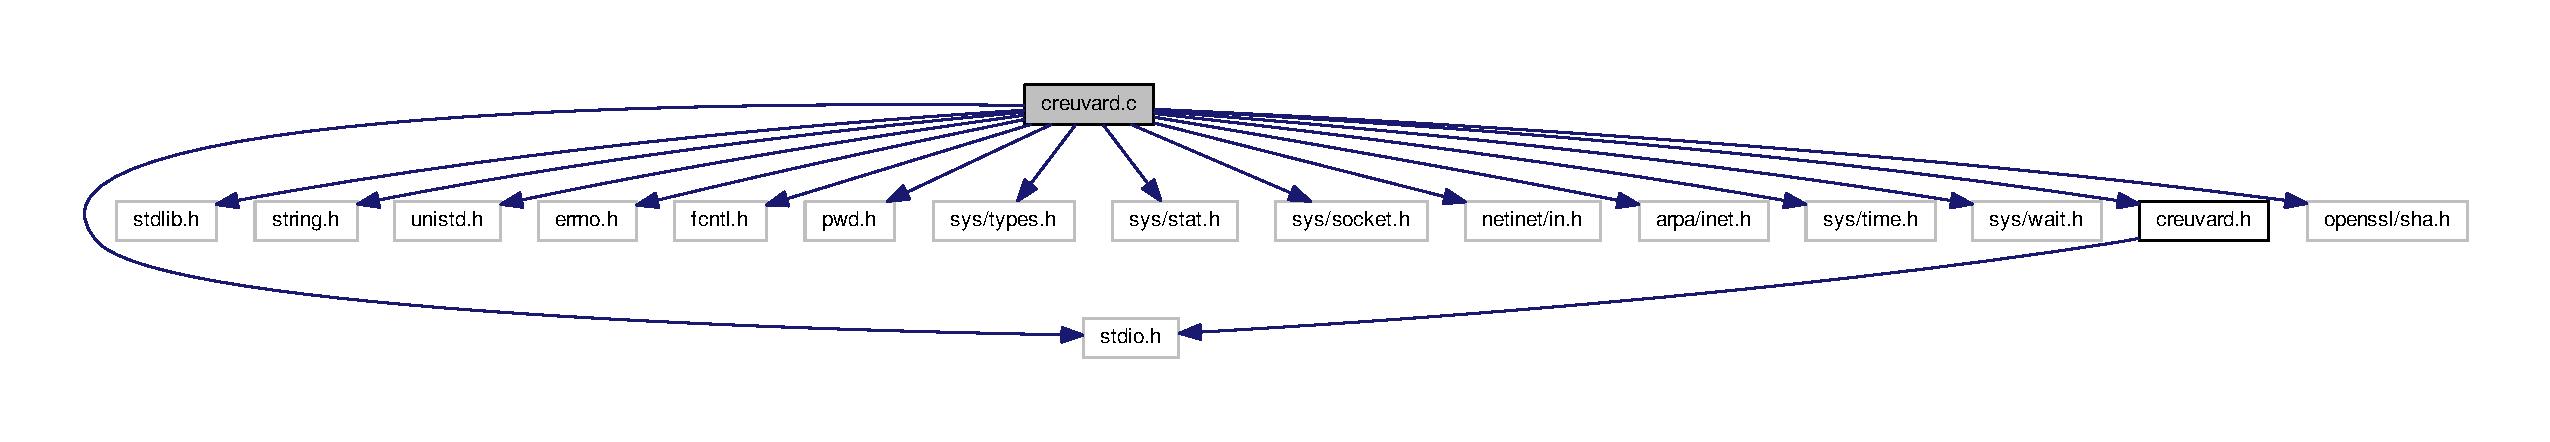
\includegraphics[width=350pt]{creuvard_8c__incl}
\end{center}
\end{figure}
\subsection*{Macros}
\begin{DoxyCompactItemize}
\item 
\hypertarget{creuvard_8c_aa8f0efe0d1ee33354f41f8898d0ee8dd}{\#define {\bfseries debug}()~fprintf(stderr, \char`\"{}D\-E\-B\-U\-G\-: fonction\-:\%s() file\-:\%s line\-:\%d\textbackslash{}n\char`\"{}, \-\_\-\-\_\-\-F\-U\-N\-C\-T\-I\-O\-N\-\_\-\-\_\-, \-\_\-\-\_\-\-F\-I\-L\-E\-\_\-\-\_\-, \-\_\-\-\_\-\-L\-I\-N\-E\-\_\-\-\_\-);}\label{creuvard_8c_aa8f0efe0d1ee33354f41f8898d0ee8dd}

\item 
\hypertarget{creuvard_8c_aeca034f67218340ecb2261a22c2f3dcd}{\#define {\bfseries B\-U\-F\-S\-I\-Z\-E}~1024$\ast$16}\label{creuvard_8c_aeca034f67218340ecb2261a22c2f3dcd}

\end{DoxyCompactItemize}
\subsection*{Fonctions}
\begin{DoxyCompactItemize}
\item 
\hypertarget{creuvard_8c_ac07d581dad1fcfa80baed0549ff86f6b}{char $\ast$ {\bfseries crv\-\_\-strdup} (const char $\ast$s)}\label{creuvard_8c_ac07d581dad1fcfa80baed0549ff86f6b}

\item 
\hypertarget{creuvard_8c_a1dfcf3da98992b56a1394e53ca8b3a5e}{void $\ast$ {\bfseries crv\-\_\-malloc} (size\-\_\-t size)}\label{creuvard_8c_a1dfcf3da98992b56a1394e53ca8b3a5e}

\item 
\hypertarget{creuvard_8c_add77ca000bcc081987558dd3e2c1df46}{void {\bfseries crv\-\_\-free} (void $\ast$ptr)}\label{creuvard_8c_add77ca000bcc081987558dd3e2c1df46}

\item 
\hypertarget{creuvard_8c_addf9cca7a0d664742f7daecf7b0e0738}{void $\ast$ {\bfseries crv\-\_\-calloc} (size\-\_\-t nmemb, size\-\_\-t size)}\label{creuvard_8c_addf9cca7a0d664742f7daecf7b0e0738}

\item 
void \hyperlink{creuvard_8c_a01e9338ce13c961896c2fc3f944899c7}{crv\-\_\-sanitise\-\_\-stdfd} (void)
\begin{DoxyCompactList}\small\item\em Ferme les descripteur de fichier. \end{DoxyCompactList}\item 
\hypertarget{creuvard_8c_a4b03e6e7431ee50171443fa86973c0cf}{F\-I\-L\-E $\ast$ {\bfseries crv\-\_\-fopen} (const char $\ast$file, const char $\ast$mode)}\label{creuvard_8c_a4b03e6e7431ee50171443fa86973c0cf}

\item 
\hypertarget{creuvard_8c_ac005199637dda040e2ac0b15dec07138}{char $\ast$$\ast$ {\bfseries crv\-\_\-cut} (const char $\ast$str, const char $\ast$separator)}\label{creuvard_8c_ac005199637dda040e2ac0b15dec07138}

\item 
\hypertarget{creuvard_8c_ad5d8198dcbaa2d875bb70cb0e78c0665}{int {\bfseries crv\-\_\-chdir} (const char $\ast$path)}\label{creuvard_8c_ad5d8198dcbaa2d875bb70cb0e78c0665}

\item 
int \hyperlink{creuvard_8c_abbcce344897d42c37a326eae7476a89a}{crv\-\_\-drop\-\_\-priv\-\_\-temp} (const char $\ast$username)
\begin{DoxyCompactList}\small\item\em Chroot le processus et donne les droits du processus. \end{DoxyCompactList}\item 
int \hyperlink{creuvard_8c_acc839f13073a1ff8a27abc9efd582a62}{crv\-\_\-restore\-\_\-priv} (void)
\begin{DoxyCompactList}\small\item\em Restaure les droits du processus avec les droits Root. \end{DoxyCompactList}\item 
\hypertarget{creuvard_8c_aa3b79f5eb9df8f74a9e858a6af48af55}{off\-\_\-t {\bfseries crv\-\_\-filesize} (const char $\ast$file)}\label{creuvard_8c_aa3b79f5eb9df8f74a9e858a6af48af55}

\item 
\hypertarget{creuvard_8c_a88ce21dfcd2abe92091f572f8d6c9a3f}{char $\ast$ {\bfseries crv\-\_\-file\-\_\-type} (const char $\ast$file)}\label{creuvard_8c_a88ce21dfcd2abe92091f572f8d6c9a3f}

\item 
\hypertarget{creuvard_8c_a95def4e27c80a6d72e3c0db1ecf55fd5}{int {\bfseries crv\-\_\-server\-\_\-listen} (int port, int nb\-\_\-pers, const char $\ast$addr, int addr\-\_\-family, int block)}\label{creuvard_8c_a95def4e27c80a6d72e3c0db1ecf55fd5}

\item 
\hypertarget{creuvard_8c_a773cf27549152fadfe4ac3ce25b2537b}{int {\bfseries crv\-\_\-set\-\_\-nonblock} (int fd)}\label{creuvard_8c_a773cf27549152fadfe4ac3ce25b2537b}

\item 
\hypertarget{creuvard_8c_a72ab0a9e7d1bacdd70e1062e75835a77}{int {\bfseries crv\-\_\-unset\-\_\-nonblock} (int fd)}\label{creuvard_8c_a72ab0a9e7d1bacdd70e1062e75835a77}

\item 
\hypertarget{creuvard_8c_af6f5886f52b1b6141e1a8545f65f14a2}{void {\bfseries crv\-\_\-daemon\-\_\-mode} (void)}\label{creuvard_8c_af6f5886f52b1b6141e1a8545f65f14a2}

\item 
\hypertarget{creuvard_8c_a0922ce5aebffd694cc7695d575a47d9f}{void {\bfseries crv\-\_\-sigchld\-\_\-handler} (int sig)}\label{creuvard_8c_a0922ce5aebffd694cc7695d575a47d9f}

\item 
\hypertarget{creuvard_8c_aa461df94e3958fd381596465d83fd790}{int {\bfseries crv\-\_\-chroot} (const char $\ast$directory)}\label{creuvard_8c_aa461df94e3958fd381596465d83fd790}

\item 
int \hyperlink{creuvard_8c_ae5abc2436ae618eba165f5c64d7a36ed}{crv\-\_\-drop\-\_\-priv\-\_\-perm\-\_\-and\-\_\-chroot} (const char $\ast$username, const char $\ast$directory)
\begin{DoxyCompactList}\small\item\em Chroot le procesus et change les permissions. \end{DoxyCompactList}\item 
\hypertarget{creuvard_8c_ad055a416845e0d653e8210b1b7934339}{size\-\_\-t {\bfseries crv\-\_\-strncpy} (char $\ast$dst, const char $\ast$src, size\-\_\-t siz)}\label{creuvard_8c_ad055a416845e0d653e8210b1b7934339}

\item 
\hypertarget{creuvard_8c_aa2a43a446ea083c713194985ee1c46a1}{size\-\_\-t {\bfseries crv\-\_\-strncat} (char $\ast$dst, const char $\ast$src, size\-\_\-t siz)}\label{creuvard_8c_aa2a43a446ea083c713194985ee1c46a1}

\item 
\hypertarget{creuvard_8c_aef5de68801c3c2bbac8b2fcd82972eb7}{off\-\_\-t {\bfseries crv\-\_\-du} (const char $\ast$file)}\label{creuvard_8c_aef5de68801c3c2bbac8b2fcd82972eb7}

\item 
\hypertarget{creuvard_8c_a0e8a276058ce74da6c72769fdc87673b}{char $\ast$ {\bfseries crv\-\_\-sha1} (const char $\ast$filename)}\label{creuvard_8c_a0e8a276058ce74da6c72769fdc87673b}

\item 
\hypertarget{creuvard_8c_a70557d2dae03678dc34f956a6a909882}{char $\ast$ {\bfseries crv\-\_\-mkstemp} (const char $\ast$prefix, const char $\ast$directory)}\label{creuvard_8c_a70557d2dae03678dc34f956a6a909882}

\item 
\hypertarget{creuvard_8c_afc499b857ede8c349d28c088ff5c902e}{int {\bfseries crv\-\_\-strncmp} (const char $\ast$s1, const char $\ast$s2)}\label{creuvard_8c_afc499b857ede8c349d28c088ff5c902e}

\item 
\hypertarget{creuvard_8c_a4c0ee6e861ac25b611a1f2d62619ec5a}{char $\ast$ {\bfseries crv\-\_\-real\-\_\-name} (const char $\ast$filename)}\label{creuvard_8c_a4c0ee6e861ac25b611a1f2d62619ec5a}

\item 
\hypertarget{creuvard_8c_add204d740cbce245703c9845dd6752a4}{char $\ast$ {\bfseries crv\-\_\-last\-\_\-dirname} (const char $\ast$path)}\label{creuvard_8c_add204d740cbce245703c9845dd6752a4}

\end{DoxyCompactItemize}


\subsection{Description détaillée}
Fonction interne. \begin{DoxyAuthor}{Auteur}
Sylvain Bourdou 
\end{DoxyAuthor}
\begin{DoxyVersion}{Version}
0.\-81 
\end{DoxyVersion}
\begin{DoxyDate}{Date}
25 Février 2013
\end{DoxyDate}
Fonction de creuvard 

\subsection{Documentation des fonctions}
\hypertarget{creuvard_8c_ae5abc2436ae618eba165f5c64d7a36ed}{\index{creuvard.\-c@{creuvard.\-c}!crv\-\_\-drop\-\_\-priv\-\_\-perm\-\_\-and\-\_\-chroot@{crv\-\_\-drop\-\_\-priv\-\_\-perm\-\_\-and\-\_\-chroot}}
\index{crv\-\_\-drop\-\_\-priv\-\_\-perm\-\_\-and\-\_\-chroot@{crv\-\_\-drop\-\_\-priv\-\_\-perm\-\_\-and\-\_\-chroot}!creuvard.c@{creuvard.\-c}}
\subsubsection[{crv\-\_\-drop\-\_\-priv\-\_\-perm\-\_\-and\-\_\-chroot}]{\setlength{\rightskip}{0pt plus 5cm}int crv\-\_\-drop\-\_\-priv\-\_\-perm\-\_\-and\-\_\-chroot (
\begin{DoxyParamCaption}
\item[{const char $\ast$}]{username, }
\item[{const char $\ast$}]{directory}
\end{DoxyParamCaption}
)}}\label{creuvard_8c_ae5abc2436ae618eba165f5c64d7a36ed}


Chroot le procesus et change les permissions. 


\begin{DoxyParams}{Paramètres}
{\em username} & Utilisateur à qui va appartenir le processus \\
\hline
{\em directory} & Répertoire dans lequel le processus va se chrooter \\
\hline
\end{DoxyParams}
\begin{DoxyReturn}{Renvoie}
-\/1 si erreur, 0 si O\-K 
\end{DoxyReturn}


Voici le graphe des appelants de cette fonction \-:
\nopagebreak
\begin{figure}[H]
\begin{center}
\leavevmode
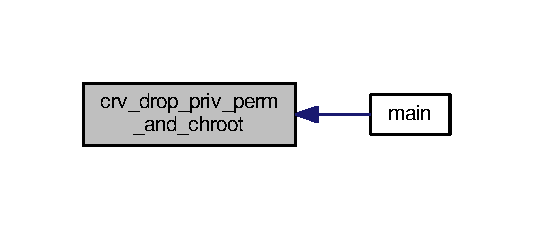
\includegraphics[width=256pt]{creuvard_8c_ae5abc2436ae618eba165f5c64d7a36ed_icgraph}
\end{center}
\end{figure}


\hypertarget{creuvard_8c_abbcce344897d42c37a326eae7476a89a}{\index{creuvard.\-c@{creuvard.\-c}!crv\-\_\-drop\-\_\-priv\-\_\-temp@{crv\-\_\-drop\-\_\-priv\-\_\-temp}}
\index{crv\-\_\-drop\-\_\-priv\-\_\-temp@{crv\-\_\-drop\-\_\-priv\-\_\-temp}!creuvard.c@{creuvard.\-c}}
\subsubsection[{crv\-\_\-drop\-\_\-priv\-\_\-temp}]{\setlength{\rightskip}{0pt plus 5cm}int crv\-\_\-drop\-\_\-priv\-\_\-temp (
\begin{DoxyParamCaption}
\item[{const char $\ast$}]{username}
\end{DoxyParamCaption}
)}}\label{creuvard_8c_abbcce344897d42c37a326eae7476a89a}


Chroot le processus et donne les droits du processus. 


\begin{DoxyParams}{Paramètres}
{\em username} & Nom de l'utilisateur utilisé \\
\hline
\end{DoxyParams}
\begin{DoxyReturn}{Renvoie}
-\/1 si erreur, 0 si O\-K 
\end{DoxyReturn}


Voici le graphe des appelants de cette fonction \-:\nopagebreak
\begin{figure}[H]
\begin{center}
\leavevmode
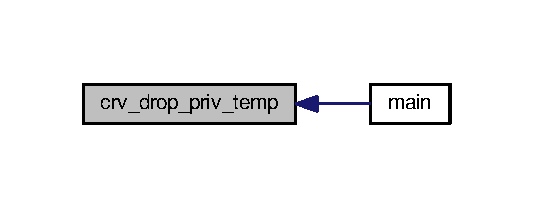
\includegraphics[width=256pt]{creuvard_8c_abbcce344897d42c37a326eae7476a89a_icgraph}
\end{center}
\end{figure}


\hypertarget{creuvard_8c_acc839f13073a1ff8a27abc9efd582a62}{\index{creuvard.\-c@{creuvard.\-c}!crv\-\_\-restore\-\_\-priv@{crv\-\_\-restore\-\_\-priv}}
\index{crv\-\_\-restore\-\_\-priv@{crv\-\_\-restore\-\_\-priv}!creuvard.c@{creuvard.\-c}}
\subsubsection[{crv\-\_\-restore\-\_\-priv}]{\setlength{\rightskip}{0pt plus 5cm}int crv\-\_\-restore\-\_\-priv (
\begin{DoxyParamCaption}
\item[{void}]{}
\end{DoxyParamCaption}
)}}\label{creuvard_8c_acc839f13073a1ff8a27abc9efd582a62}


Restaure les droits du processus avec les droits Root. 


\begin{DoxyParams}{Paramètres}
{\em \textbackslash{}return} & -\/1 si erreur, 0 si O\-K \\
\hline
\end{DoxyParams}


Voici le graphe des appelants de cette fonction \-:\nopagebreak
\begin{figure}[H]
\begin{center}
\leavevmode
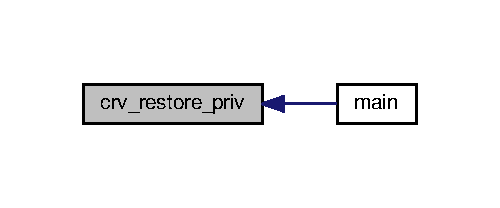
\includegraphics[width=240pt]{creuvard_8c_acc839f13073a1ff8a27abc9efd582a62_icgraph}
\end{center}
\end{figure}


\hypertarget{creuvard_8c_a01e9338ce13c961896c2fc3f944899c7}{\index{creuvard.\-c@{creuvard.\-c}!crv\-\_\-sanitise\-\_\-stdfd@{crv\-\_\-sanitise\-\_\-stdfd}}
\index{crv\-\_\-sanitise\-\_\-stdfd@{crv\-\_\-sanitise\-\_\-stdfd}!creuvard.c@{creuvard.\-c}}
\subsubsection[{crv\-\_\-sanitise\-\_\-stdfd}]{\setlength{\rightskip}{0pt plus 5cm}void crv\-\_\-sanitise\-\_\-stdfd (
\begin{DoxyParamCaption}
\item[{void}]{}
\end{DoxyParamCaption}
)}}\label{creuvard_8c_a01e9338ce13c961896c2fc3f944899c7}


Ferme les descripteur de fichier. 


\begin{DoxyParams}{Paramètres}
{\em } & \\
\hline
\end{DoxyParams}


Voici le graphe des appelants de cette fonction \-:\nopagebreak
\begin{figure}[H]
\begin{center}
\leavevmode
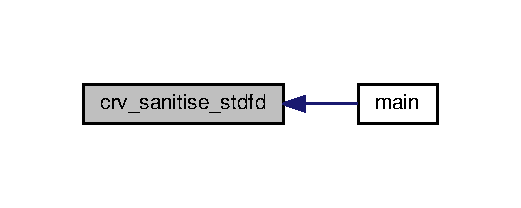
\includegraphics[width=250pt]{creuvard_8c_a01e9338ce13c961896c2fc3f944899c7_icgraph}
\end{center}
\end{figure}



\hypertarget{creuvuxd_8c}{\section{Référence du fichier creuvuxd.\-c}
\label{creuvuxd_8c}\index{creuvuxd.\-c@{creuvuxd.\-c}}
}


Fichier principale.  


{\ttfamily \#include $<$stdlib.\-h$>$}\\*
{\ttfamily \#include $<$string.\-h$>$}\\*
{\ttfamily \#include $<$unistd.\-h$>$}\\*
{\ttfamily \#include $<$limits.\-h$>$}\\*
{\ttfamily \#include $<$errno.\-h$>$}\\*
{\ttfamily \#include $<$pwd.\-h$>$}\\*
{\ttfamily \#include $<$fcntl.\-h$>$}\\*
{\ttfamily \#include $<$termios.\-h$>$}\\*
{\ttfamily \#include $<$sys/types.\-h$>$}\\*
{\ttfamily \#include $<$sys/socket.\-h$>$}\\*
{\ttfamily \#include $<$sys/stat.\-h$>$}\\*
{\ttfamily \#include $<$sys/wait.\-h$>$}\\*
{\ttfamily \#include $<$netinet/in.\-h$>$}\\*
{\ttfamily \#include $<$arpa/inet.\-h$>$}\\*
{\ttfamily \#include $<$sqlite3.\-h$>$}\\*
{\ttfamily \#include \char`\"{}creuvard.\-h\char`\"{}}\\*
{\ttfamily \#include \char`\"{}server\-\_\-conf.\-h\char`\"{}}\\*
{\ttfamily \#include \char`\"{}help.\-h\char`\"{}}\\*
{\ttfamily \#include \char`\"{}network.\-h\char`\"{}}\\*
{\ttfamily \#include \char`\"{}create\-\_\-database.\-h\char`\"{}}\\*
Graphe des dépendances par inclusion de creuvuxd.\-c\-:\nopagebreak
\begin{figure}[H]
\begin{center}
\leavevmode
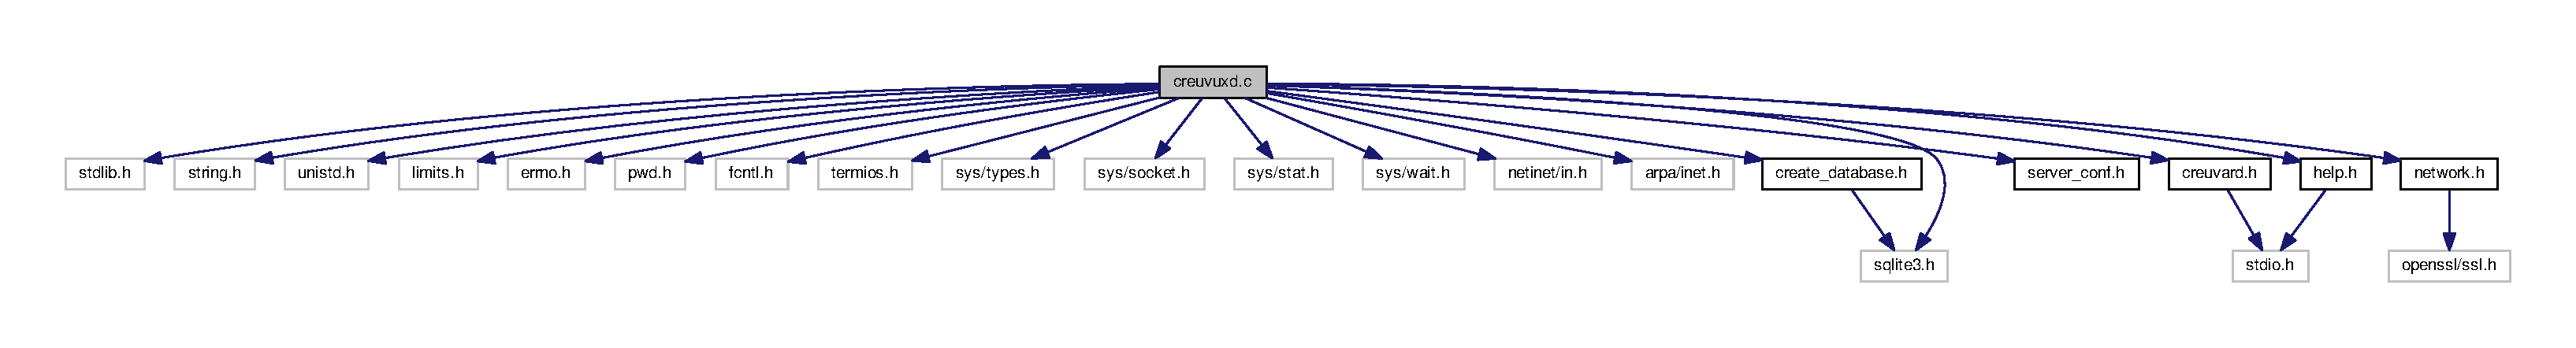
\includegraphics[width=350pt]{creuvuxd_8c__incl}
\end{center}
\end{figure}
\subsection*{Fonctions}
\begin{DoxyCompactItemize}
\item 
int \hyperlink{creuvuxd_8c_a3c04138a5bfe5d72780bb7e82a18e627}{main} (int argc, char $\ast$$\ast$argv)
\begin{DoxyCompactList}\small\item\em Fonction principale. \end{DoxyCompactList}\end{DoxyCompactItemize}
\subsection*{Variables}
\begin{DoxyCompactItemize}
\item 
\hypertarget{creuvuxd_8c_a4dd19b7d2f1d9097a32e6e523087a598}{\hyperlink{struct_server_options}{Server\-Options} {\bfseries options}}\label{creuvuxd_8c_a4dd19b7d2f1d9097a32e6e523087a598}

\end{DoxyCompactItemize}


\subsection{Description détaillée}
Fichier principale. \begin{DoxyAuthor}{Auteur}
Sylvain Bourdou 
\end{DoxyAuthor}
\begin{DoxyVersion}{Version}
0.\-81 
\end{DoxyVersion}
\begin{DoxyDate}{Date}
25 Février 2013
\end{DoxyDate}
Création d'un serveur 

\subsection{Documentation des fonctions}
\hypertarget{creuvuxd_8c_a3c04138a5bfe5d72780bb7e82a18e627}{\index{creuvuxd.\-c@{creuvuxd.\-c}!main@{main}}
\index{main@{main}!creuvuxd.c@{creuvuxd.\-c}}
\subsubsection[{main}]{\setlength{\rightskip}{0pt plus 5cm}int main (
\begin{DoxyParamCaption}
\item[{int}]{argc, }
\item[{char $\ast$$\ast$}]{argv}
\end{DoxyParamCaption}
)}}\label{creuvuxd_8c_a3c04138a5bfe5d72780bb7e82a18e627}


Fonction principale. 


\begin{DoxyParams}{Paramètres}
{\em argv} & Argument passés en ligne de commande \\
\hline
\end{DoxyParams}
\begin{DoxyReturn}{Renvoie}
-\/1 en cas d'erreur, et 0 si tout va bien. 
\end{DoxyReturn}


Voici le graphe d'appel pour cette fonction \-:
\nopagebreak
\begin{figure}[H]
\begin{center}
\leavevmode
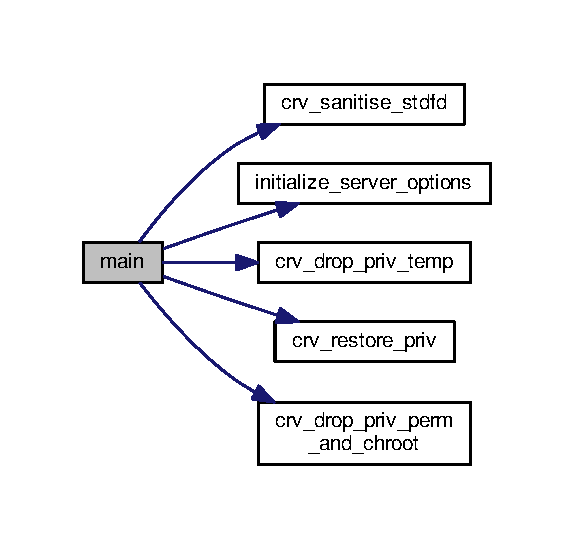
\includegraphics[width=276pt]{creuvuxd_8c_a3c04138a5bfe5d72780bb7e82a18e627_cgraph}
\end{center}
\end{figure}



\hypertarget{server__conf_8c}{\section{Référence du fichier server\-\_\-conf.\-c}
\label{server__conf_8c}\index{server\-\_\-conf.\-c@{server\-\_\-conf.\-c}}
}


Fichier contenant 2 fonctions de configurations du serveur.  


{\ttfamily \#include $<$string.\-h$>$}\\*
{\ttfamily \#include $<$sys/types.\-h$>$}\\*
{\ttfamily \#include $<$sys/socket.\-h$>$}\\*
{\ttfamily \#include \char`\"{}server\-\_\-conf.\-h\char`\"{}}\\*
{\ttfamily \#include \char`\"{}creuvard.\-h\char`\"{}}\\*
Graphe des dépendances par inclusion de server\-\_\-conf.\-c\-:\nopagebreak
\begin{figure}[H]
\begin{center}
\leavevmode
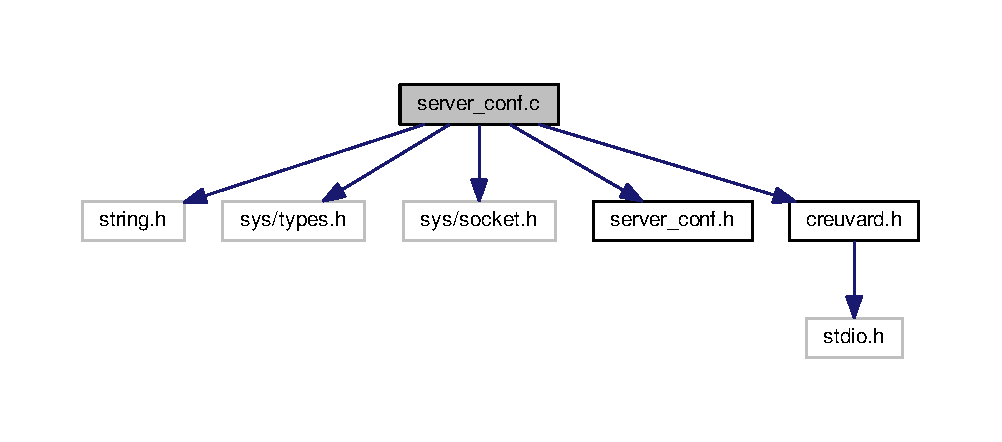
\includegraphics[width=350pt]{server__conf_8c__incl}
\end{center}
\end{figure}
\subsection*{Macros}
\begin{DoxyCompactItemize}
\item 
\hypertarget{server__conf_8c_aa8f0efe0d1ee33354f41f8898d0ee8dd}{\#define {\bfseries debug}()~fprintf(stderr, \char`\"{}D\-E\-B\-U\-G\-: fonction\-:\%s() file\-:\%s line\-:\%d\textbackslash{}n\char`\"{}, \-\_\-\-\_\-\-F\-U\-N\-C\-T\-I\-O\-N\-\_\-\-\_\-, \-\_\-\-\_\-\-F\-I\-L\-E\-\_\-\-\_\-, \-\_\-\-\_\-\-L\-I\-N\-E\-\_\-\-\_\-);}\label{server__conf_8c_aa8f0efe0d1ee33354f41f8898d0ee8dd}

\end{DoxyCompactItemize}
\subsection*{Fonctions}
\begin{DoxyCompactItemize}
\item 
void \hyperlink{server__conf_8c_ab7c4ca9e8fb899188488d87cbe8691ea}{initialize\-\_\-server\-\_\-options} (\hyperlink{struct_server_options}{Server\-Options} $\ast$options)
\begin{DoxyCompactList}\small\item\em Initialise les options du serveur. \end{DoxyCompactList}\item 
\hypertarget{server__conf_8c_a16545ecc34797329bf6602782882a068}{void {\bfseries Free\-\_\-options} (void)}\label{server__conf_8c_a16545ecc34797329bf6602782882a068}

\end{DoxyCompactItemize}
\subsection*{Variables}
\begin{DoxyCompactItemize}
\item 
\hypertarget{server__conf_8c_a4dd19b7d2f1d9097a32e6e523087a598}{\hyperlink{struct_server_options}{Server\-Options} {\bfseries options}}\label{server__conf_8c_a4dd19b7d2f1d9097a32e6e523087a598}

\end{DoxyCompactItemize}


\subsection{Description détaillée}
Fichier contenant 2 fonctions de configurations du serveur. \begin{DoxyAuthor}{Auteur}
Sylvain Bourdou 
\end{DoxyAuthor}
\begin{DoxyVersion}{Version}
0.\-81 
\end{DoxyVersion}
\begin{DoxyDate}{Date}
25 Février 2013
\end{DoxyDate}
Fonction de creuvard 

\subsection{Documentation des fonctions}
\hypertarget{server__conf_8c_ab7c4ca9e8fb899188488d87cbe8691ea}{\index{server\-\_\-conf.\-c@{server\-\_\-conf.\-c}!initialize\-\_\-server\-\_\-options@{initialize\-\_\-server\-\_\-options}}
\index{initialize\-\_\-server\-\_\-options@{initialize\-\_\-server\-\_\-options}!server_conf.c@{server\-\_\-conf.\-c}}
\subsubsection[{initialize\-\_\-server\-\_\-options}]{\setlength{\rightskip}{0pt plus 5cm}void initialize\-\_\-server\-\_\-options (
\begin{DoxyParamCaption}
\item[{{\bf Server\-Options} $\ast$}]{options}
\end{DoxyParamCaption}
)}}\label{server__conf_8c_ab7c4ca9e8fb899188488d87cbe8691ea}


Initialise les options du serveur. 


\begin{DoxyParams}{Paramètres}
{\em options} & Struct contenant toutes les variables d'environement. \\
\hline
\end{DoxyParams}


Voici le graphe des appelants de cette fonction \-:\nopagebreak
\begin{figure}[H]
\begin{center}
\leavevmode
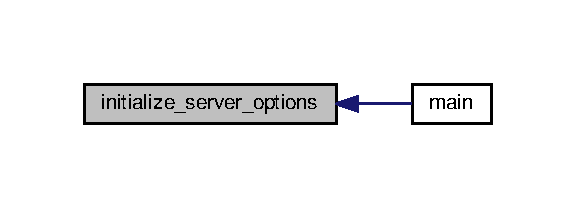
\includegraphics[width=276pt]{server__conf_8c_ab7c4ca9e8fb899188488d87cbe8691ea_icgraph}
\end{center}
\end{figure}



\addcontentsline{toc}{part}{Index}
\printindex
\end{document}
